
\documentclass[aspectratio=169]{beamer}
\usetheme{Madrid}
 
\usepackage{graphicx}
%\usepackage[spanish]{babel}
\usepackage[utf8]{inputenc}
\usepackage{hyperref}
\usepackage{verbatim}

%\setbeamertemplate{footline}[frame number]

\AtBeginSection[]
{
	\begin{frame}
		\frametitle{Table of Contents}
		\tableofcontents[currentsection]
	\end{frame}
}



\begin{document}


\title{Introduction to neural networks}  
\subtitle{The perceptron} 
\author[J.I. Vasquez]{\textbf{Juan Irving Vásquez} \\jivg.org}
\date{\today \copyright}
\institute[jivg.org]{Centro de Innovación y Desarrollo Tecnológico en Cómputo \\ Instituto Politécnico Nacional}
% logo of my university
\titlegraphic{
\includegraphics[height=1.2cm]{ipn-cidetec.png}\hspace{0.1cm}
\includegraphics[height=1.2cm]{escudoESCOM}}
\frame{\titlepage} 

%%%%%%%%%%%%%%%%%%%%%%%%%%%%%%%%%%%%%%%%%%%%%%%%%%%%%%%%

\frame{
	\frametitle{Contents}
\tableofcontents
}


\section{Data representation}


\begin{frame}
	\frametitle{Dataset}
	\begin{columns}[c] % opción [t] alinea arriba, [c] centra, [b] abajo
		% Columna izquierda
		\begin{column}{0.48\textwidth}
			A dataset is a set of tuples,
			\begin{equation}
				\mathcal{D} = \left\lbrace  (X^1, y^1) \dots (X^\mu, y^\mu) \dots (X^m, y^m) \right\rbrace 
			\end{equation}
			where $X$ is an input such as an image, and $y$ is the ground truth.
		\end{column}
		% Columna derecha
		\begin{column}{0.40\textwidth}
			\pause
			%\begin{center}
			\includegraphics[height=0.8\textheight]{"ChatGPT Image Sep 1, 2025, 12_58_53 PM"} 
			\\
			{\small "Frases que René Descartes nunca dijo".}
			%\end{center}
		\end{column}
	\end{columns}
\end{frame}



\begin{frame}
	\frametitle{Dataset implementation}
	\begin{center}
		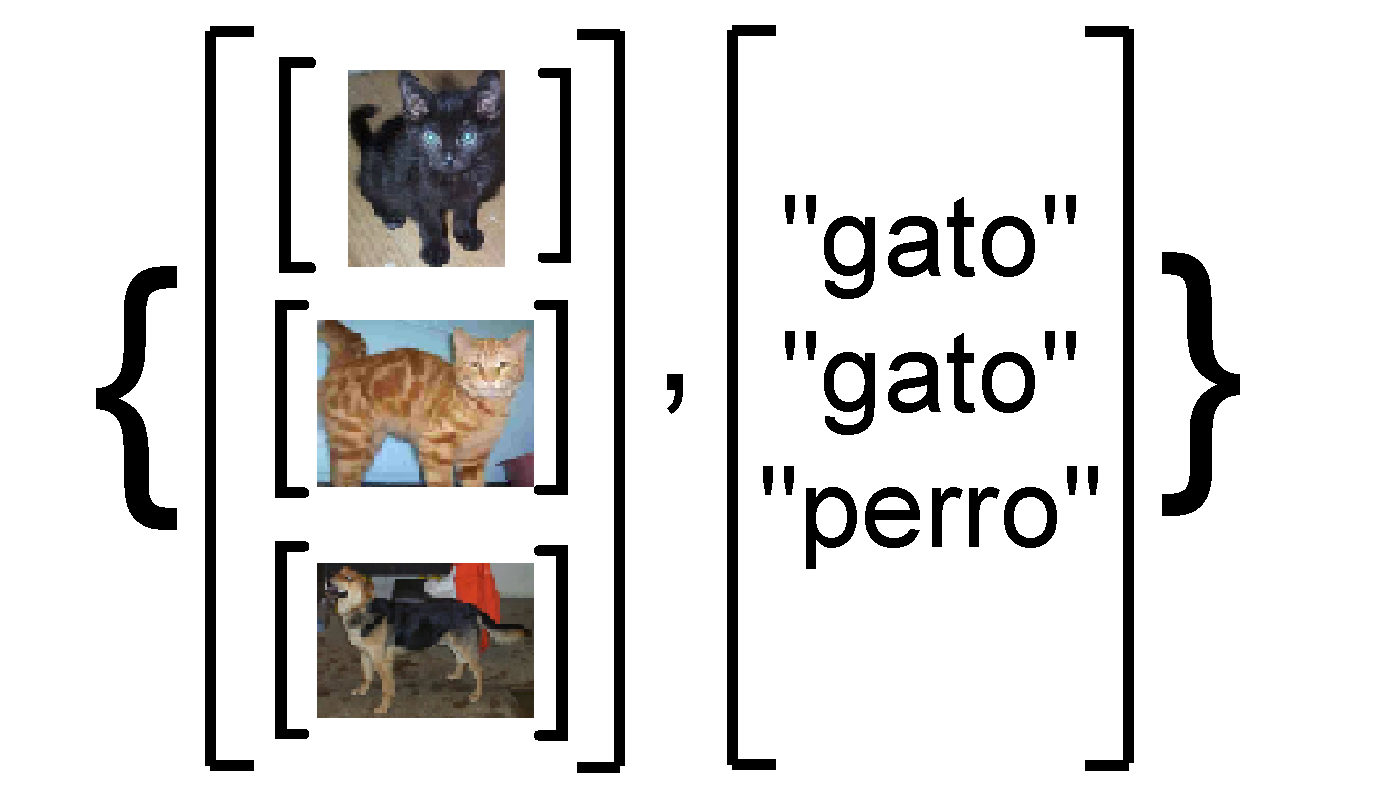
\includegraphics[height=0.4\textheight]{dataset.drawio}
	\end{center}
	
	\begin{equation}
		\mathcal{D} = \left\lbrace 
		\begin{bmatrix}
			x^{1}_{1} & \dots & x^{1}_{n} \\
			\vdots & \ddots & \vdots \\
			x^{m}_{1} & \dots & x^{m}_{n}
		\end{bmatrix},
		\begin{bmatrix}
			y^1	\\
			\vdots \\
			y^m
		\end{bmatrix} \right\rbrace 
	\end{equation}
	where for the inputs, $X$, each row is a example and the columns are features of each example, and for the targets, $Y$, each element is the target label of that example.
	
\end{frame} 


\begin{frame}
	\frametitle{Dataset}
	In some ocasions, we will write:
	\begin{equation}
		\mathcal{D} = \left\lbrace 
		\begin{bmatrix}
			X^\mu
		\end{bmatrix},
		\begin{bmatrix}
			Y^\mu
		\end{bmatrix} \right\rbrace 
	\end{equation}
\end{frame}


\section{The perceptron}

\frame{
	\frametitle{The problem}
	\begin{columns}
		% Left Column: Text and Equations
		\begin{column}{0.5\textwidth}
			\begin{itemize}
				\item We want a machine, $f$, so that, it says 'yes' when something is detected, namely
					\begin{equation}
						y \leftarrow f(X)
					\end{equation}
			\end{itemize}
		\end{column}
		
		% Right Column: Image
		\begin{column}{0.5\textwidth}
			\centering
			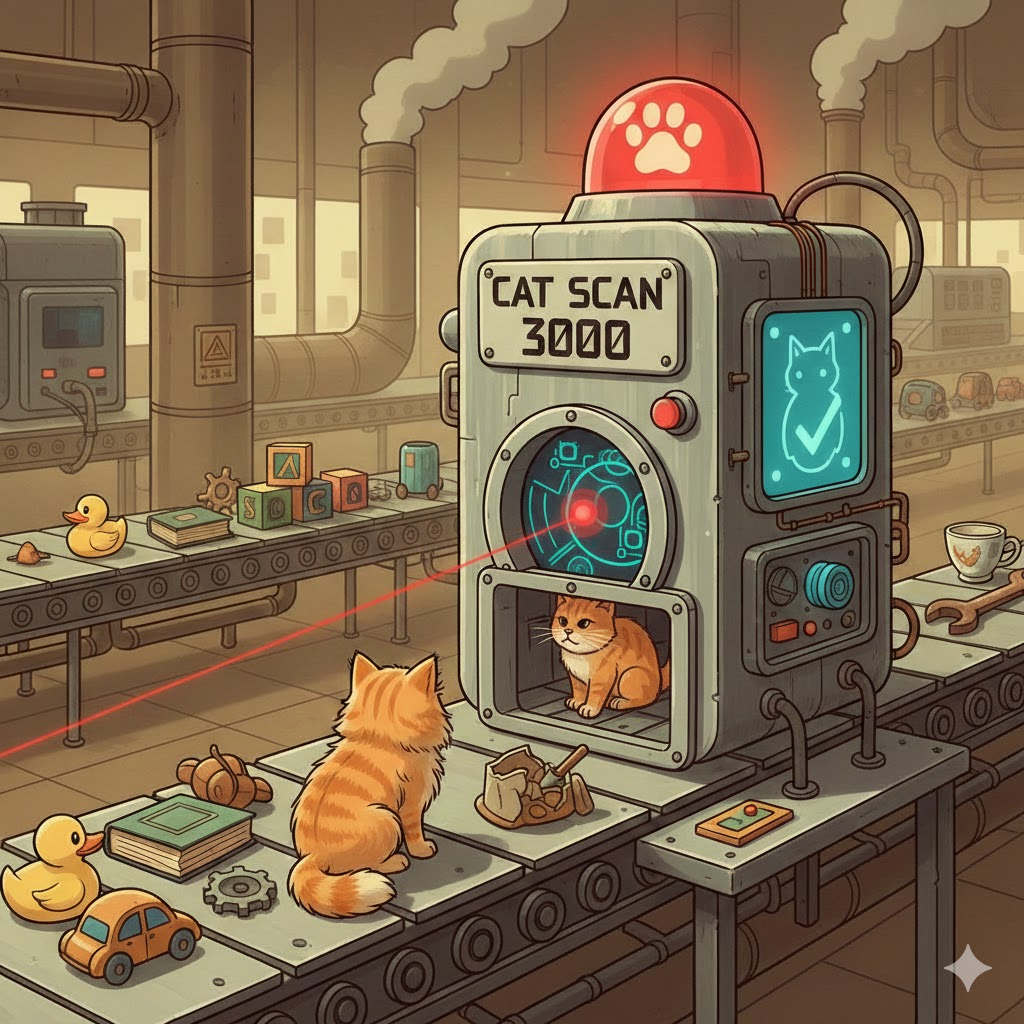
\includegraphics[width=0.75\textwidth]{catscan}
			% Replace 'your-image-file' with the name of your cat-machine illustration
		\end{column}
	\end{columns}
}


\frame{
	\frametitle{Frank Rosenblatt}
	\begin{figure}
		\centering
		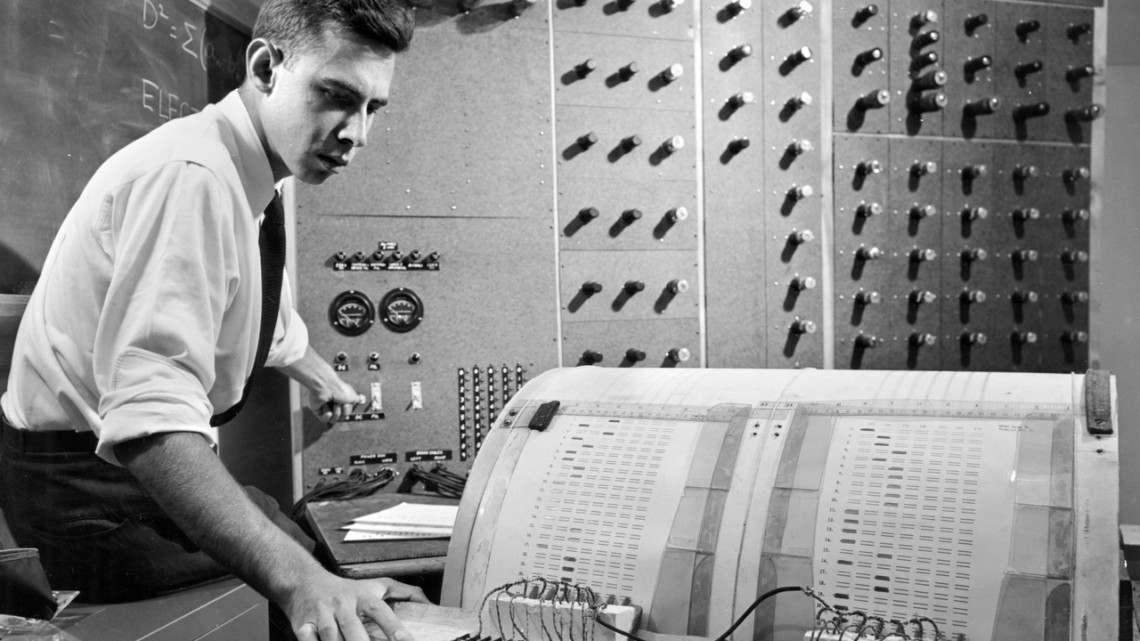
\includegraphics[width=0.65\linewidth]{0925_rosenblatt_main}
		\caption{Frank Rosenblatt ’50, Ph.D. ’56, works on the “perceptron”\footnote{\tiny https://news.cornell.edu/stories/2019/09/professors-perceptron-paved-way-ai-60-years-too-soon}}
		\label{fig:0925rosenblattmain}
	\end{figure}
}


\frame{
	\frametitle{Neuron}
	\begin{figure}
		\centering
		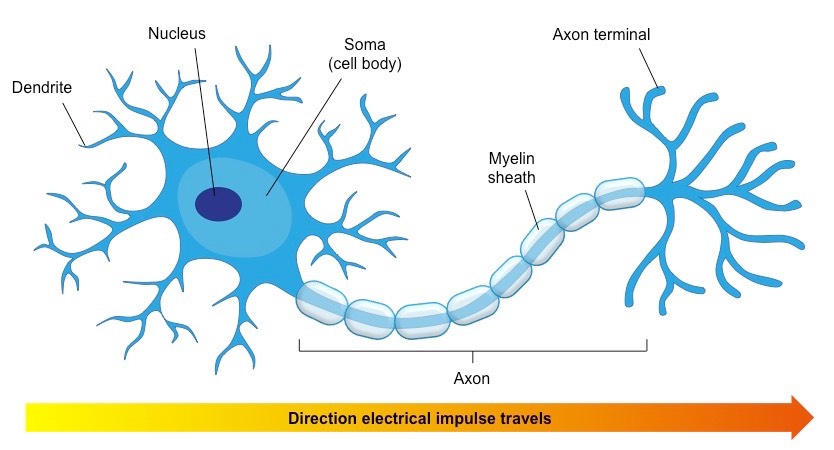
\includegraphics[width=0.7\linewidth]{neuron_med}
		%	\caption{}
		\label{fig:neuronmed}
	\end{figure}
	
}


\frame{
	\frametitle{Perceptron}
	%\framesubtitle{}
	\begin{figure}
		\centering
		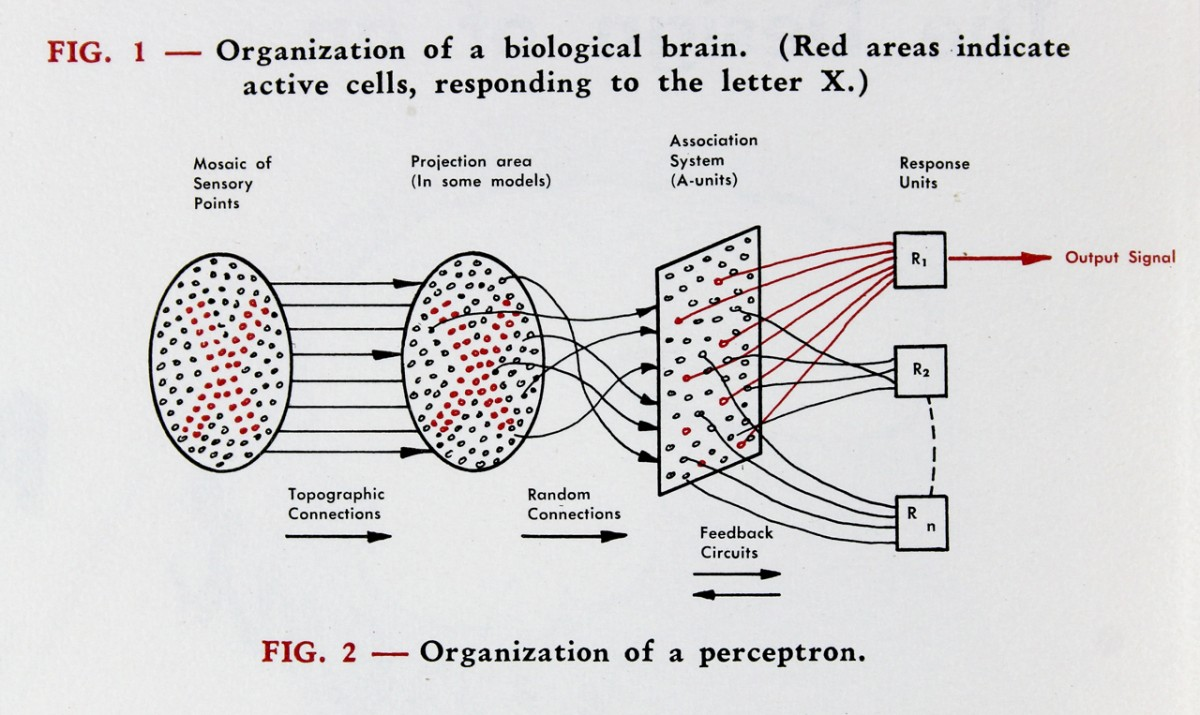
\includegraphics[width=0.7\linewidth]{0925_rosenblatt4}
		\caption{“The Design of an Intelligent Automaton,” Summer 1958}
		\label{fig:0925rosenblatt4}
	\end{figure}
}




\frame{
	\frametitle{Perceptron}
	
	\begin{itemize}
		\item “Yet we are about to witness the birth of such a machine – a machine capable of perceiving, recognizing and identifying its surroundings without any human training or control.” Rosenblatt
		\item ``It is a mathematical function mapping some set of input values to output values"
		%\item It resembles to a neuron
		%\item How does it take a decision?
	\end{itemize}
	
	\begin{figure}
		\centering
		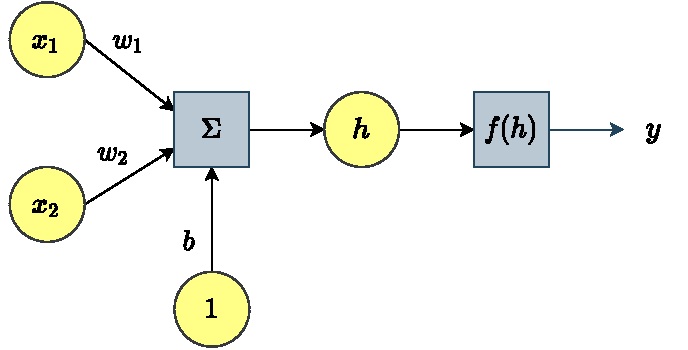
\includegraphics[height=0.4\textheight]{simple_nn}
		\caption{Perceptron (Extended diagram)}
		\label{fig:simplenn}
	\end{figure}	
}


\frame{
	\frametitle{Perceptron}
	%\framesubtitle{Weights}
	\begin{itemize}
		\item Weights. Each input to a perceptron has an associated weight that represents its importance. 
		\begin{equation}
		h = \sum_{i=1}^{n} w_i \cdot x_i + b
		\end{equation}
		\begin{equation}
			\hat{y} = f(h)
		\end{equation}
		%\begin{figure}
		%\centering
		%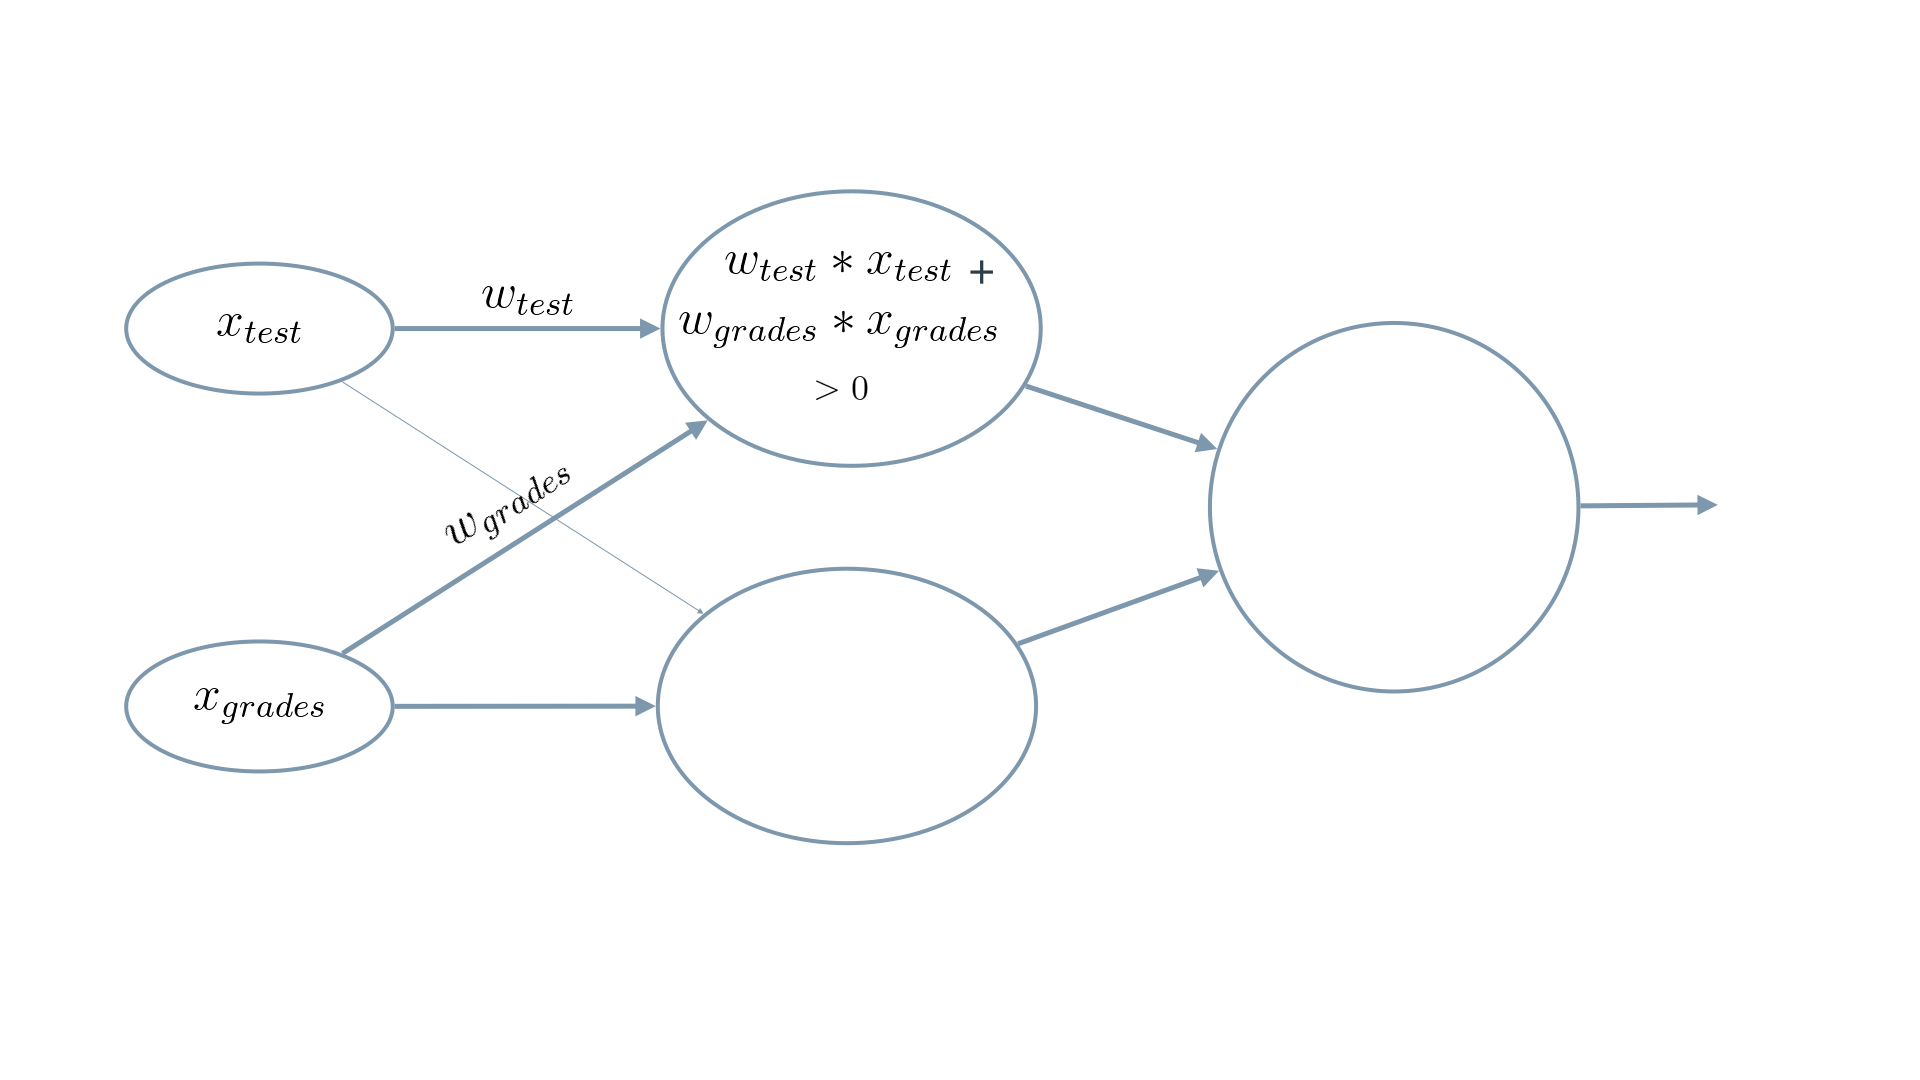
\includegraphics[height=0.5\textheight]{./perceptron-graphics001}
		%\end{figure}
	\end{itemize}
	\begin{figure}
		\centering
		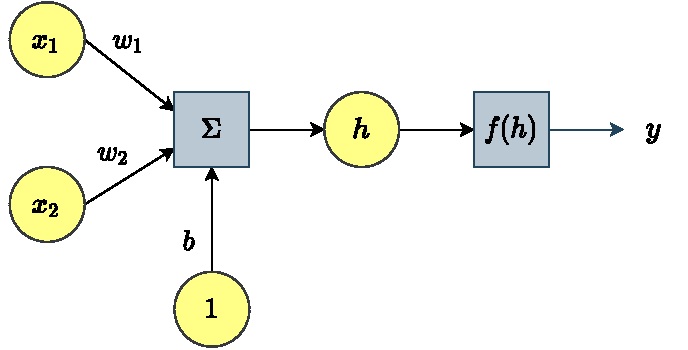
\includegraphics[height=0.4\textheight]{simple_nn}
		\caption{Perceptron}
		\label{fig:simplenn}
	\end{figure}
}


\frame{
	\frametitle{Perceptron}
	\framesubtitle{Activation function}
	\begin{itemize}
		\item Activation function $f(h)$. 
		
		\item Heaviside or step function.
		\begin{center}
			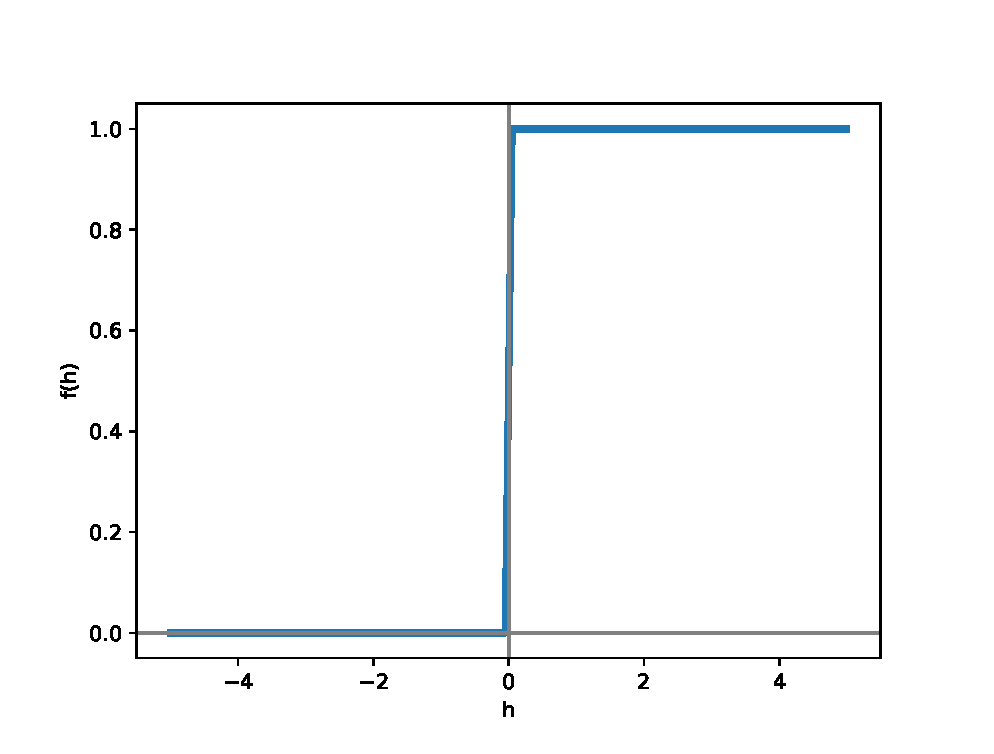
\includegraphics[height=0.6\textheight]{./step_function}
		\end{center}
	\end{itemize}
}


%\frame{
%	\frametitle{RELU}
%	\begin{itemize}
%		\item Rectified linear unit
%		$$y = max(0,x)$$
%		\begin{center}
%			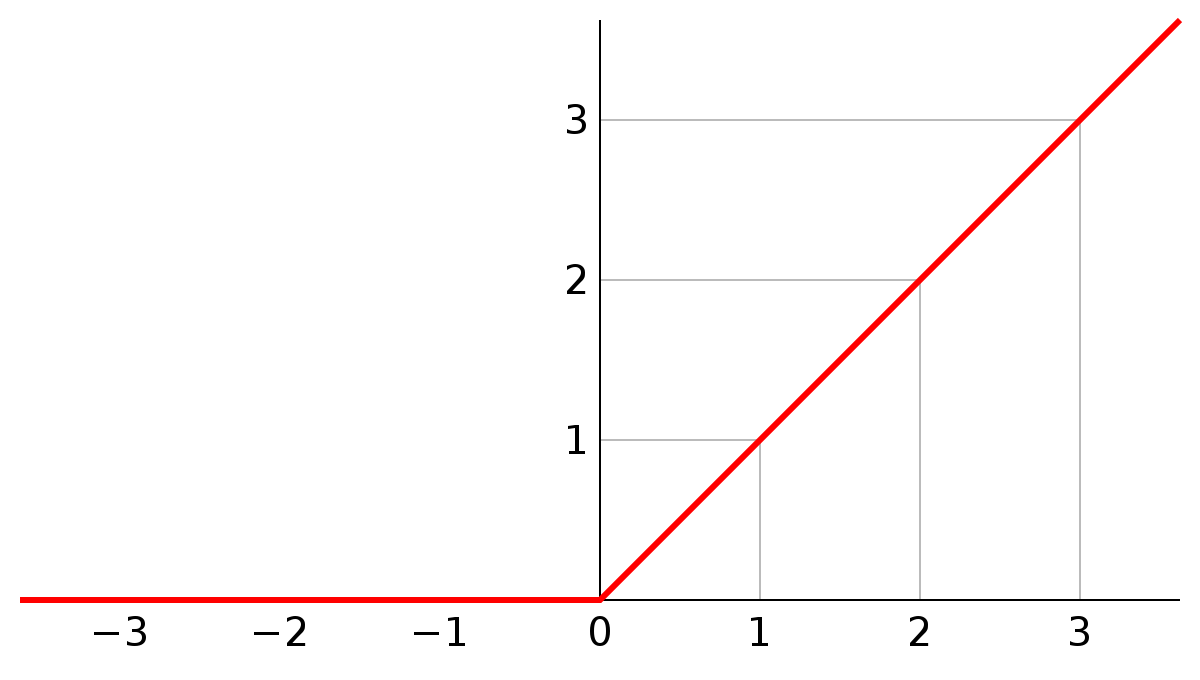
\includegraphics[width=0.7\linewidth]{./relu}
%		\end{center}
%		\item Derivative?
%	\end{itemize}
%}




\frame{
	\frametitle{Perceptron}
	\framesubtitle{Bias}
	\begin{itemize}
		\item One way to get our function to return 1 for more inputs is to add a value to the results of our linear combination, called a bias.
		\begin{center}
			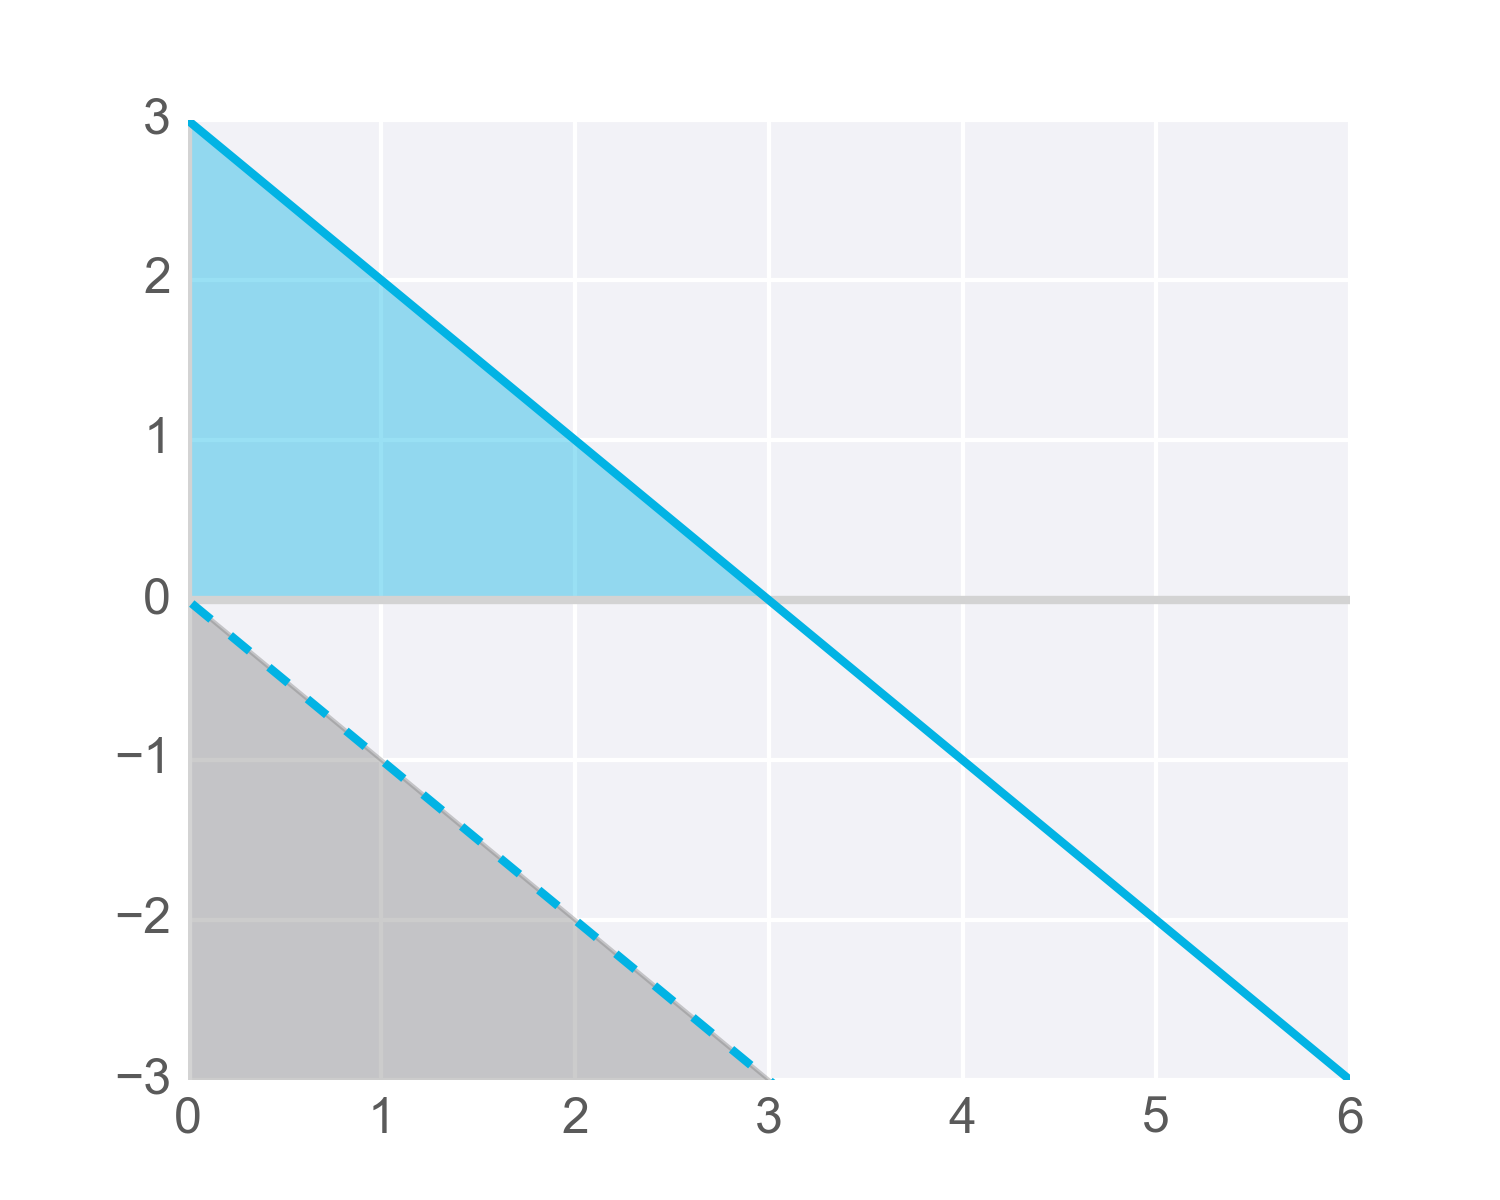
\includegraphics[height=0.5\textheight]{./example-after-bias}
		\end{center}
		
	\end{itemize}
}


\frame{
	\frametitle{Perceptron}
	\begin{itemize}
		\item Full perceptron formula:
		\begin{equation}
		f(x_1,x_2,\dots,x_n) = \begin{cases}
		0 & \text{if } \sum w_i \cdot x_i + b < 0 \\
		1 & \text{if } \sum w_i \cdot x_i + b \geq 0
		\end{cases}	
		\end{equation}
		
	\end{itemize}
	\begin{figure}
		\centering
		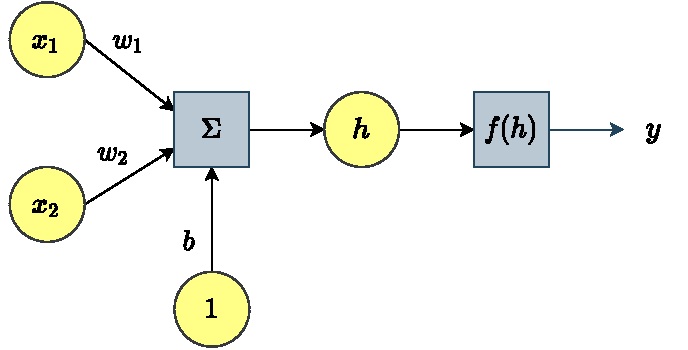
\includegraphics[height=0.4\textheight]{simple_nn}
		\caption{Perceptron}
		\label{fig:simplenn}
	\end{figure}
}


\begin{frame}
\frametitle{Comparion against MyP model}
\begin{itemize}
	\item Perceptron (Rosenblatt)
	\begin{equation}
		f(x_1, \dots, x_n): \mathbb{
			R}^n \rightarrow \{0,1\}
	\end{equation}
	\item MyP (McCulloch y Pitts)
	\begin{equation}
		f(x_1, \dots, x_n): \{0, 1\}^n \rightarrow \{0,1\}
	\end{equation}
\end{itemize}
\end{frame}


\frame{
\frametitle{Amount of parameters}
	The amount of parameters is given by the sum of weights plus biases per layer.
	\begin{equation}
		\Phi = \{ w_1 \dots w_n, b \}
	\end{equation}
	\begin{equation}
		|\Phi| = n + 1
	\end{equation}
}


%\frame{
%\frametitle{Perceptron - Quiz}
%\begin{itemize}
%\item What are the weights and bias for the AND perceptron?
%\item Download the code: \\
%\url{https://github.com/irvingvasquez/cv2course_intro_nn.git}
%\end{itemize}
%}


%\frame{
%	\frametitle{Excercise}
%	\begin{itemize}
%		\item Build a perceptron for constructing the following functions: 
%		
%		\begin{itemize}
%			\item Or 
%			\item And 
%			\item Not
%		\end{itemize}
%	\end{itemize}
%}


%\frame{
%	\frametitle{References}
%	\begin{itemize}
%		\item Goodfellow, Ian, et al. Deep learning. Vol. 1. Cambridge: MIT press, 2016.
%		\item Udacity - Self Driving Car Nanodegree
%		\item Udacity - Introduction to Computer Vision 
%		\item Khan Academy
%	\end{itemize}
%}




\section{Learning rule}


\begin{frame}
\frametitle{Learning problem}
Given the perceptron and the targets:

\begin{equation}
	Y \approx f(\textcolor{red}{W}X+b) ?
\end{equation}

\begin{block}{Problem}
How do we automatically get the parameters of the perceptron so that the behaviour in a dataset will be replicated?
\end{block}
\end{frame}




\begin{frame}
\frametitle{What to chose?}

\begin{columns}
	
	% First column
	\begin{column}{0.48\textwidth}
		\begin{figure}
			\centering
			\includegraphics[height=0.6\textheight]{"ChatGPT Image Sep 1, 2025, 04_27_32 PM"}
			\caption{Where do we want to go?}
			\label{fig:chatgpt-image-sep-1-2025-042732-pm}
		\end{figure}
	\end{column}
	\pause
	% Second column
	\begin{column}{0.48\textwidth}
		\begin{itemize}
			\item We want to diminish the total error. We will write it as the loss funcion.
			\begin{equation}
				\mathcal{L} = SAE = \sum_\mu | y^\mu - \hat{y}^\mu |
			\end{equation}		
		\item Each error will guide us (left or right):
		\begin{equation}
			e^\mu = y^\mu - \hat{y}^\mu
		\end{equation}	
		\end{itemize}
	\end{column}
	
\end{columns}

\end{frame}



\begin{frame}
\frametitle{Perceptron learning rule \footnote{Hassoun, Mohamad H. Fundamentals of artificial neural networks. MIT press, 1995.}}
For a single example:
\begin{itemize}
	\item Initial step
	\begin{equation}
		W^0 = [r_1, \dots, r_n] | r_i \sim \mathcal{U}(a,b)
	\end{equation}
	\item Repeat
	\begin{equation}
		W^{t+1} = W^{t} + \eta (y - \hat{y}) X,
	\end{equation} where $\eta > 0$. $\eta$ is called learning rate. $X$ actuates like a "responsable" of the output.
\end{itemize}
\end{frame}



\begin{frame}
	\frametitle{Perceptron learning rule \footnote{Rosenblatt, Frank. Principles of neurodynamics: Perceptrons and the theory of brain mechanisms. Vol. 55. Washington, DC: Spartan books, 1962.} \footnote{Hassoun, Mohamad H. Fundamentals of artificial neural networks. MIT press, 1995.}}
	For a \textbf{dataset} $D$:
	\begin{enumerate}
		\item Initial step
		\begin{equation}
			W^0 = [r_1, \dots, r_n] | r_i \sim \mathcal{U}(a,b)
		\end{equation}
		\item Repeat
		\begin{equation}
			W^{t+1} = W^{t} + \eta (Y^{t} - \hat{Y}^{t}) \mathcal{D},
		\end{equation} where $\eta > 0$. 
	\end{enumerate}
\end{frame}


%\frame{
%	\frametitle{A net of decisions}
%	\begin{figure}
%		\centering
%		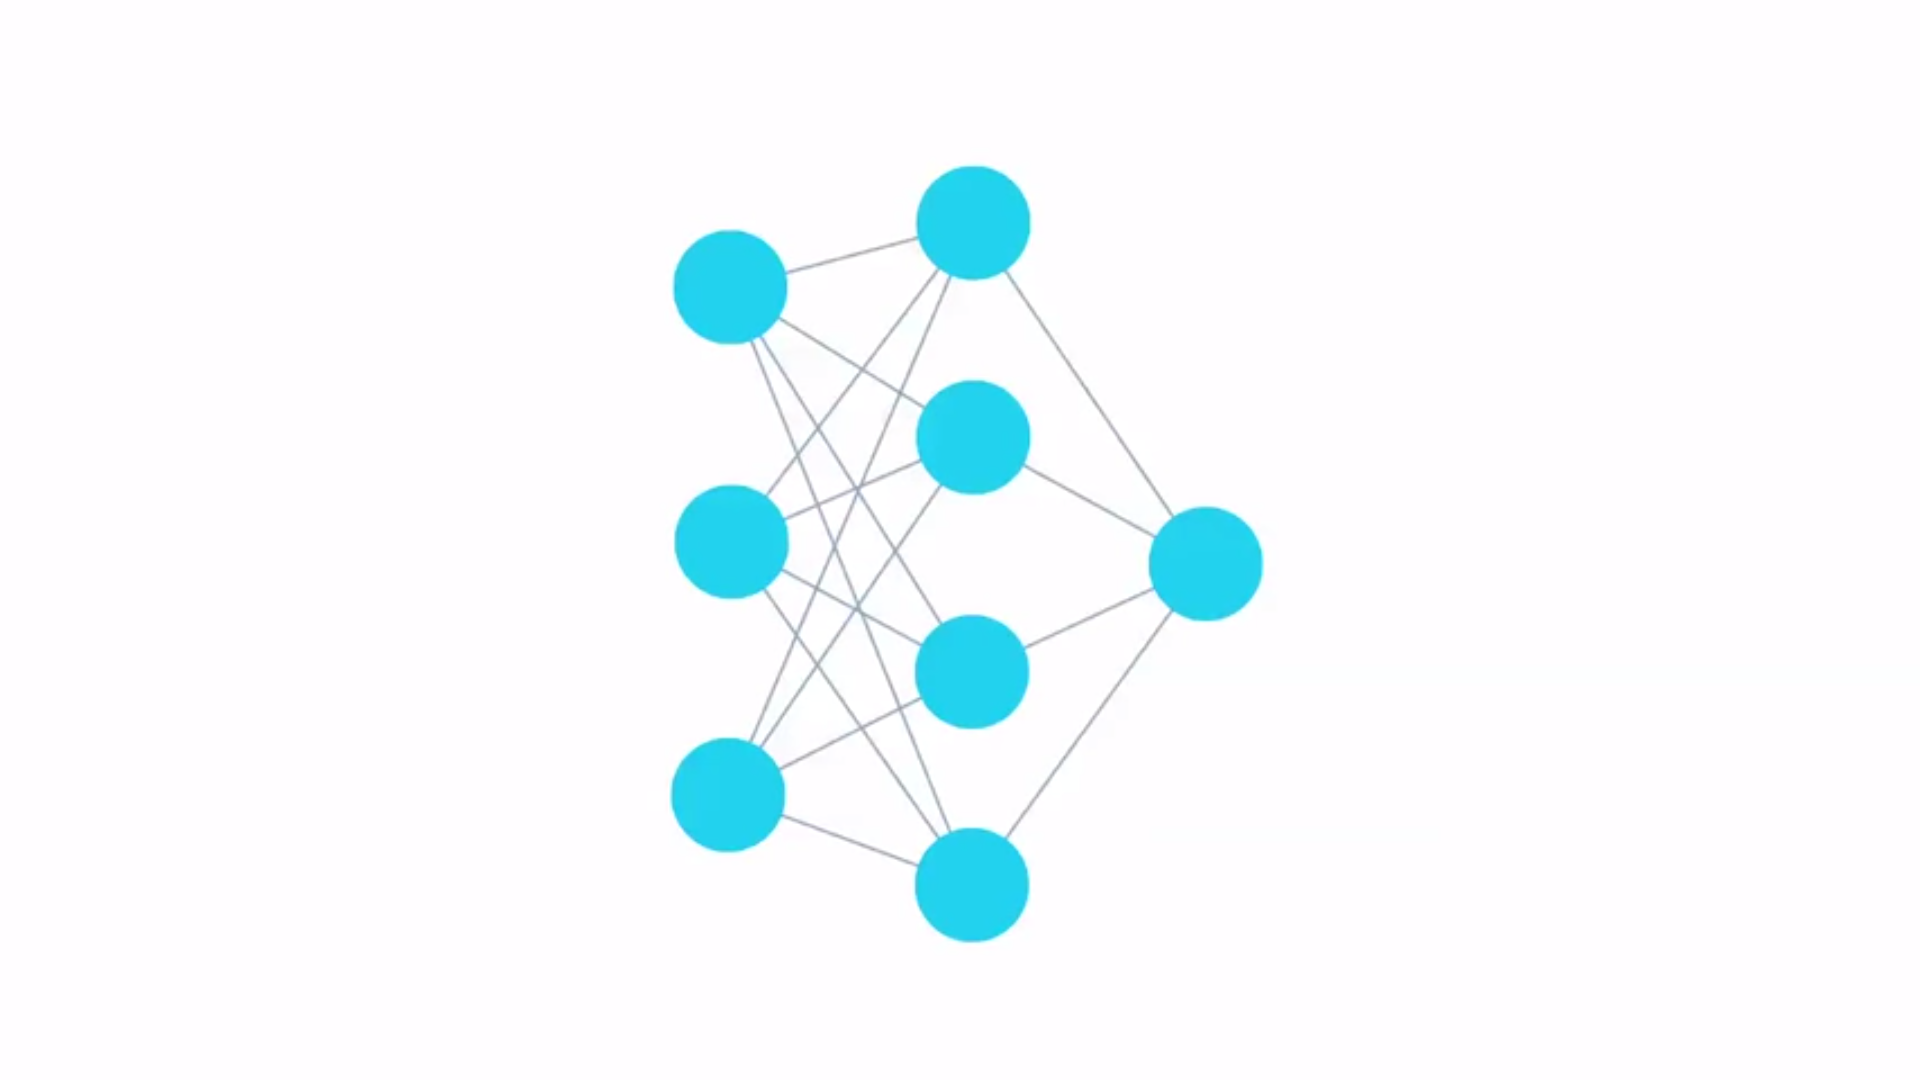
\includegraphics[height=0.7\textheight]{./logreg30}
%	\end{figure}
%}
%
%
%\frame{
%	\frametitle{Neural Network}
%	\begin{figure}
%		\centering
%		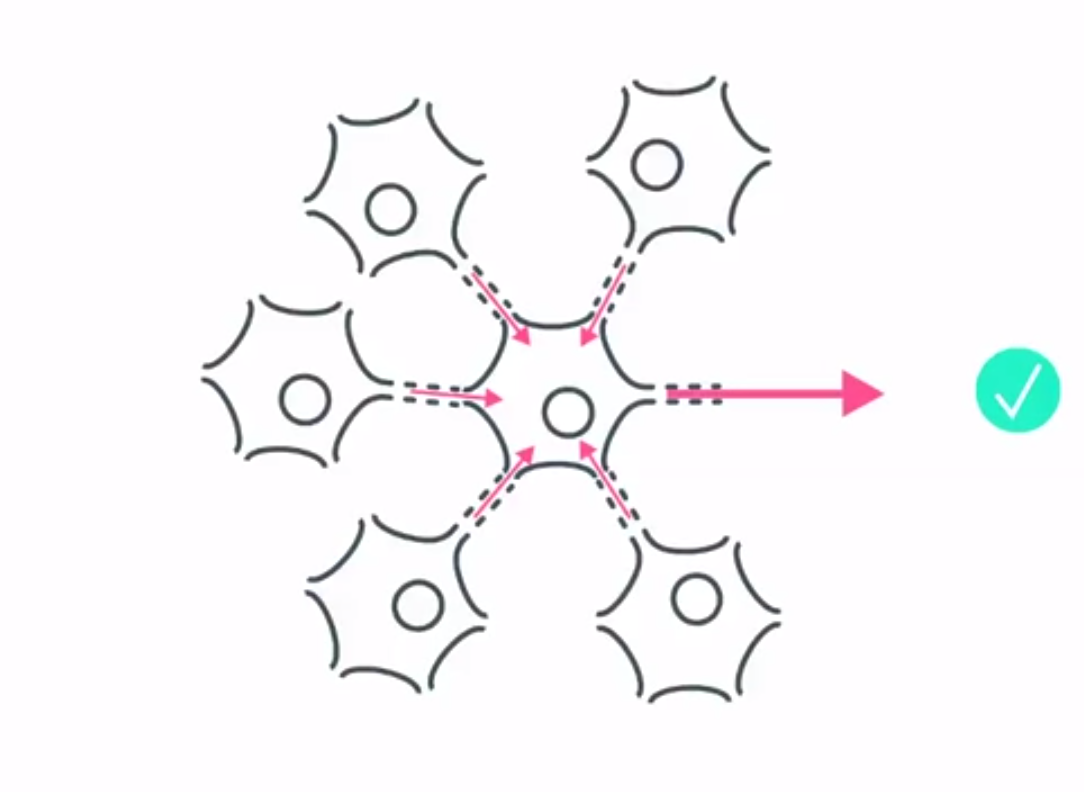
\includegraphics[height=0.7\textheight]{./logreg31}
%	\end{figure}
%}


\begin{frame}
\frametitle{Activities}
\begin{itemize}
	\item Primer equipo exponer: Widrow, Bernard. Adaptive "ADALINE" Neuron Using Chemical memistors. 1960.
\end{itemize}
\end{frame}


\frame{
	\frametitle{References}
	\begin{thebibliography}{9}

		
		\bibitem{einstein} 
		Albert Einstein. 
		\textit{Zur Elektrodynamik bewegter K{\"o}rper}. (German) 
		[\textit{On the electrodynamics of moving bodies}]. 
		Annalen der Physik, 322(10):891–921, 1905.
		
		\bibitem{knuthwebsite} 
		Knuth: Computers and Typesetting,
		\\\texttt{http://www-cs-faculty.stanford.edu/\~{}uno/abcde.html}
		
		\bibitem{joshi2016opencv}
		Joshi, Prateek and Escriv{\'a}, David Mill{\'a}n and Godoy, Vinicius,
		Packt Publishing Ltd, 2016
		
		%@book{joshi2016opencv,
		%	title={OpenCV By Example},
		%	author={Joshi, Prateek and Escriv{\'a}, David Mill{\'a}n and Godoy, Vinicius},
		%	year={2016},
		%	publisher={Packt Publishing Ltd}
		%}
		
		\bibitem{figuraNeurona}
		\url{https://ib.bioninja.com.au/standard-level/topic-6-human-physiology/65-neurons-and-synapses/neurons.html}
		
		\bibitem{walpole}
		Walpole, R. E., Myers, R. H., Myers, S. L., \& Ye, K. Probability and statistics for engineers and scientists (9th Ed). New York: Macmillan.
		
	\end{thebibliography}
}


\end{document}